\documentclass{article}
\usepackage{natbib}
\usepackage{amsmath}
\usepackage{graphicx}
\graphicspath{ {./images/} } 

\title{Happywhale - Whale and Dolphin Identification}
\author{Matthew Harding}
\date{April 2024}

\begin{document}

\maketitle

\section{Introduction}
This project explores the problem of classifiying images of dolphin and whales to identify indivduals. This work 
is based on the \emph{Happywhale - Whale and Dolphin Identification} Kaggle competition \cite{kaggle_comp}.

Data for this competition contains over 50,000 images of over 15,000 unique individual marine mammals from 30 different species collected from 28 different research organizations. 
Individuals have been manually identified and given an individual\_id by marine researchers.

Unlike a typical classification problem in which there is a fixed set of classes which examples of all classes within the training data, this problem required the ability to classify individuals not contained within the training dataset.

\section{Training Data}

\begin{figure}[!htb]
    \centering
    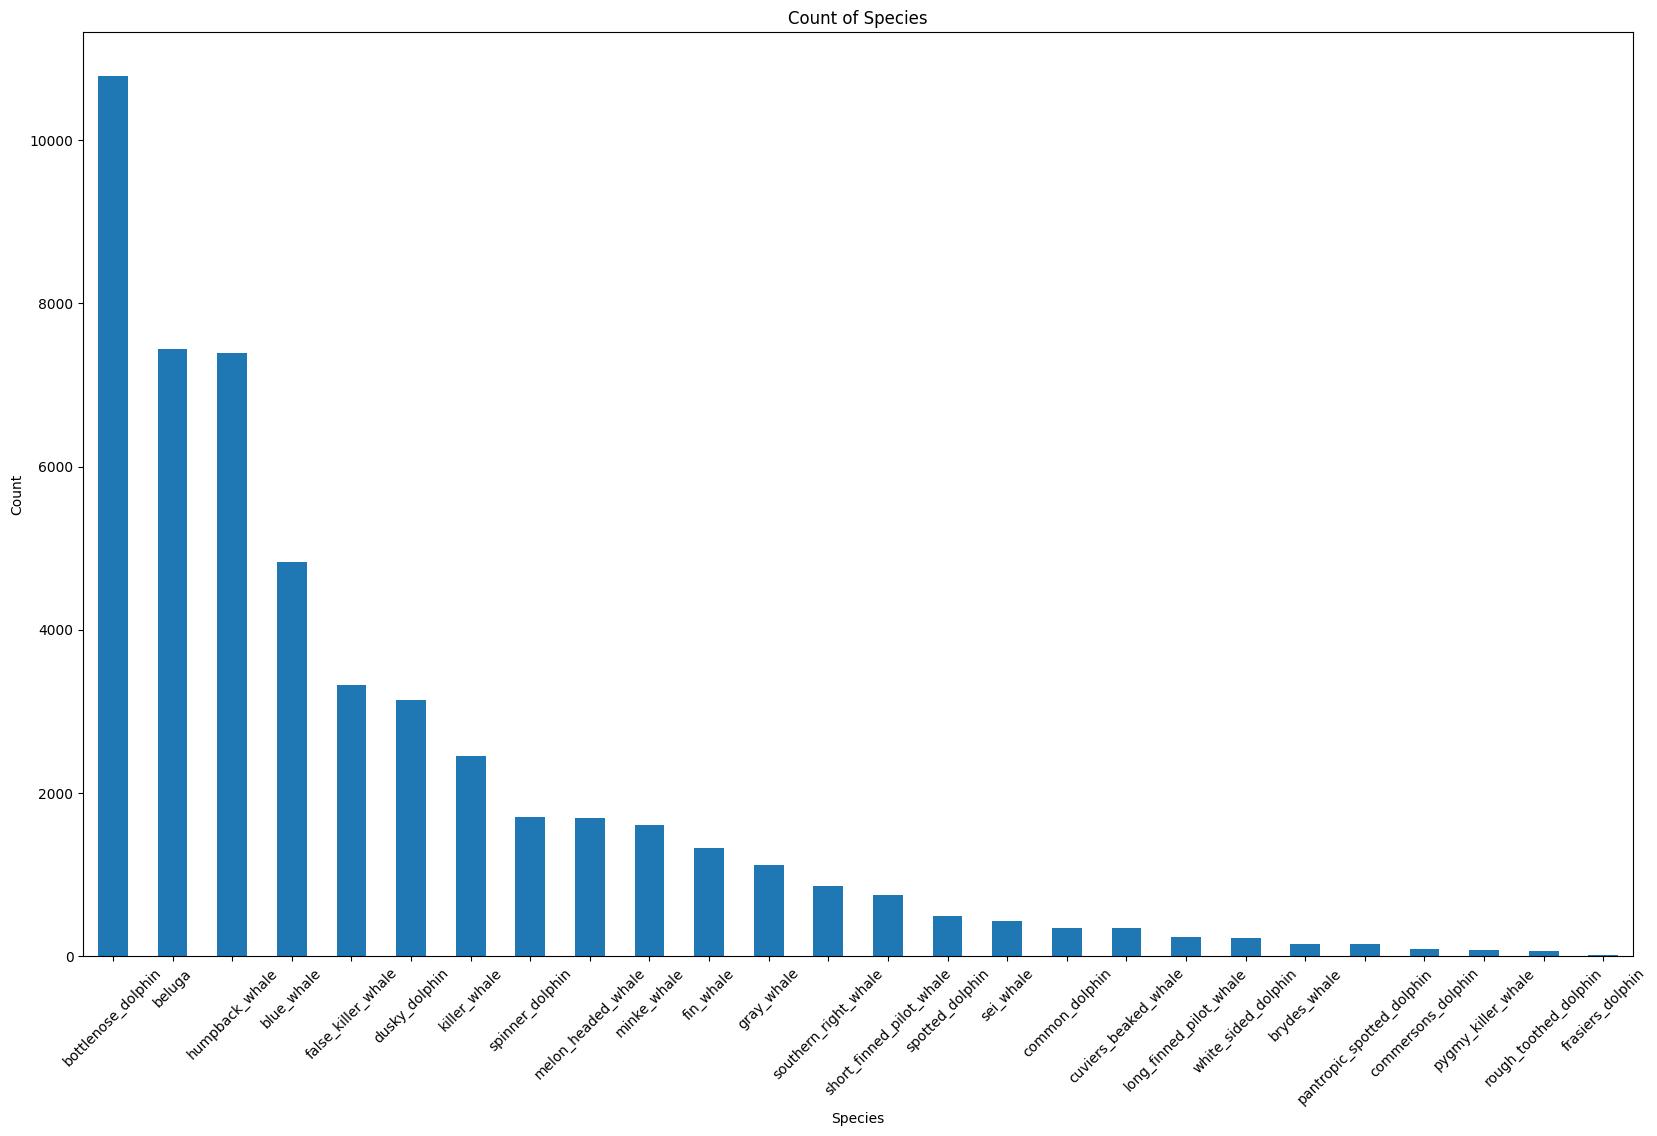
\includegraphics[width=0.8\textwidth]{species_histogram.png}
    \caption{Number of training images per species}
    \label{fig:species_count_histogram}
\end{figure}

\begin{figure}[!htb]
    \centering
    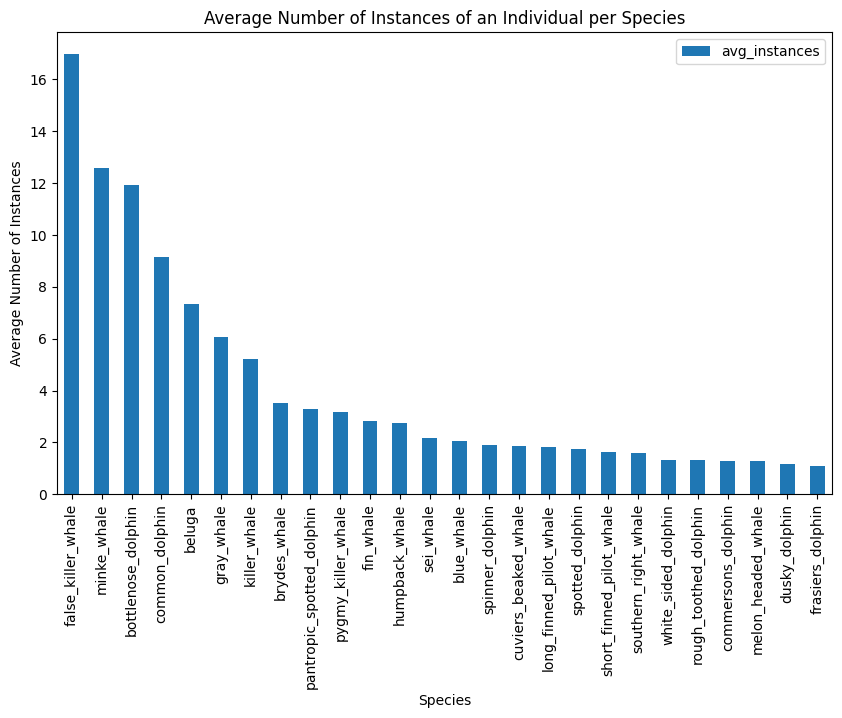
\includegraphics[width=0.8\textwidth]{mean_individuals_histogram.png}
    \caption{Mean count of images per individual by species}
    \label{fig:individual_mean_count_histogram}
\end{figure}

Looking at the histogram of species Figure \ref{fig:species_count_histogram}, there is a clear inbalance in the number of images per species with the vast majority
of labelled images being for bottlenose dolphins, beluga whales, humpback whales and blue whales. For some species the number of examples it so low it will be difficult to gain a high level of accuracy within classification.

Figure \ref{fig:individual_mean_count_histogram} shows the mean count of images per indivdual by species where we see another imbalance with some species on average containing a large number of images per indivudal whilst others only contain one or two images per individual.


\section{Image Preprocessing}

\begin{figure}
    \centering
    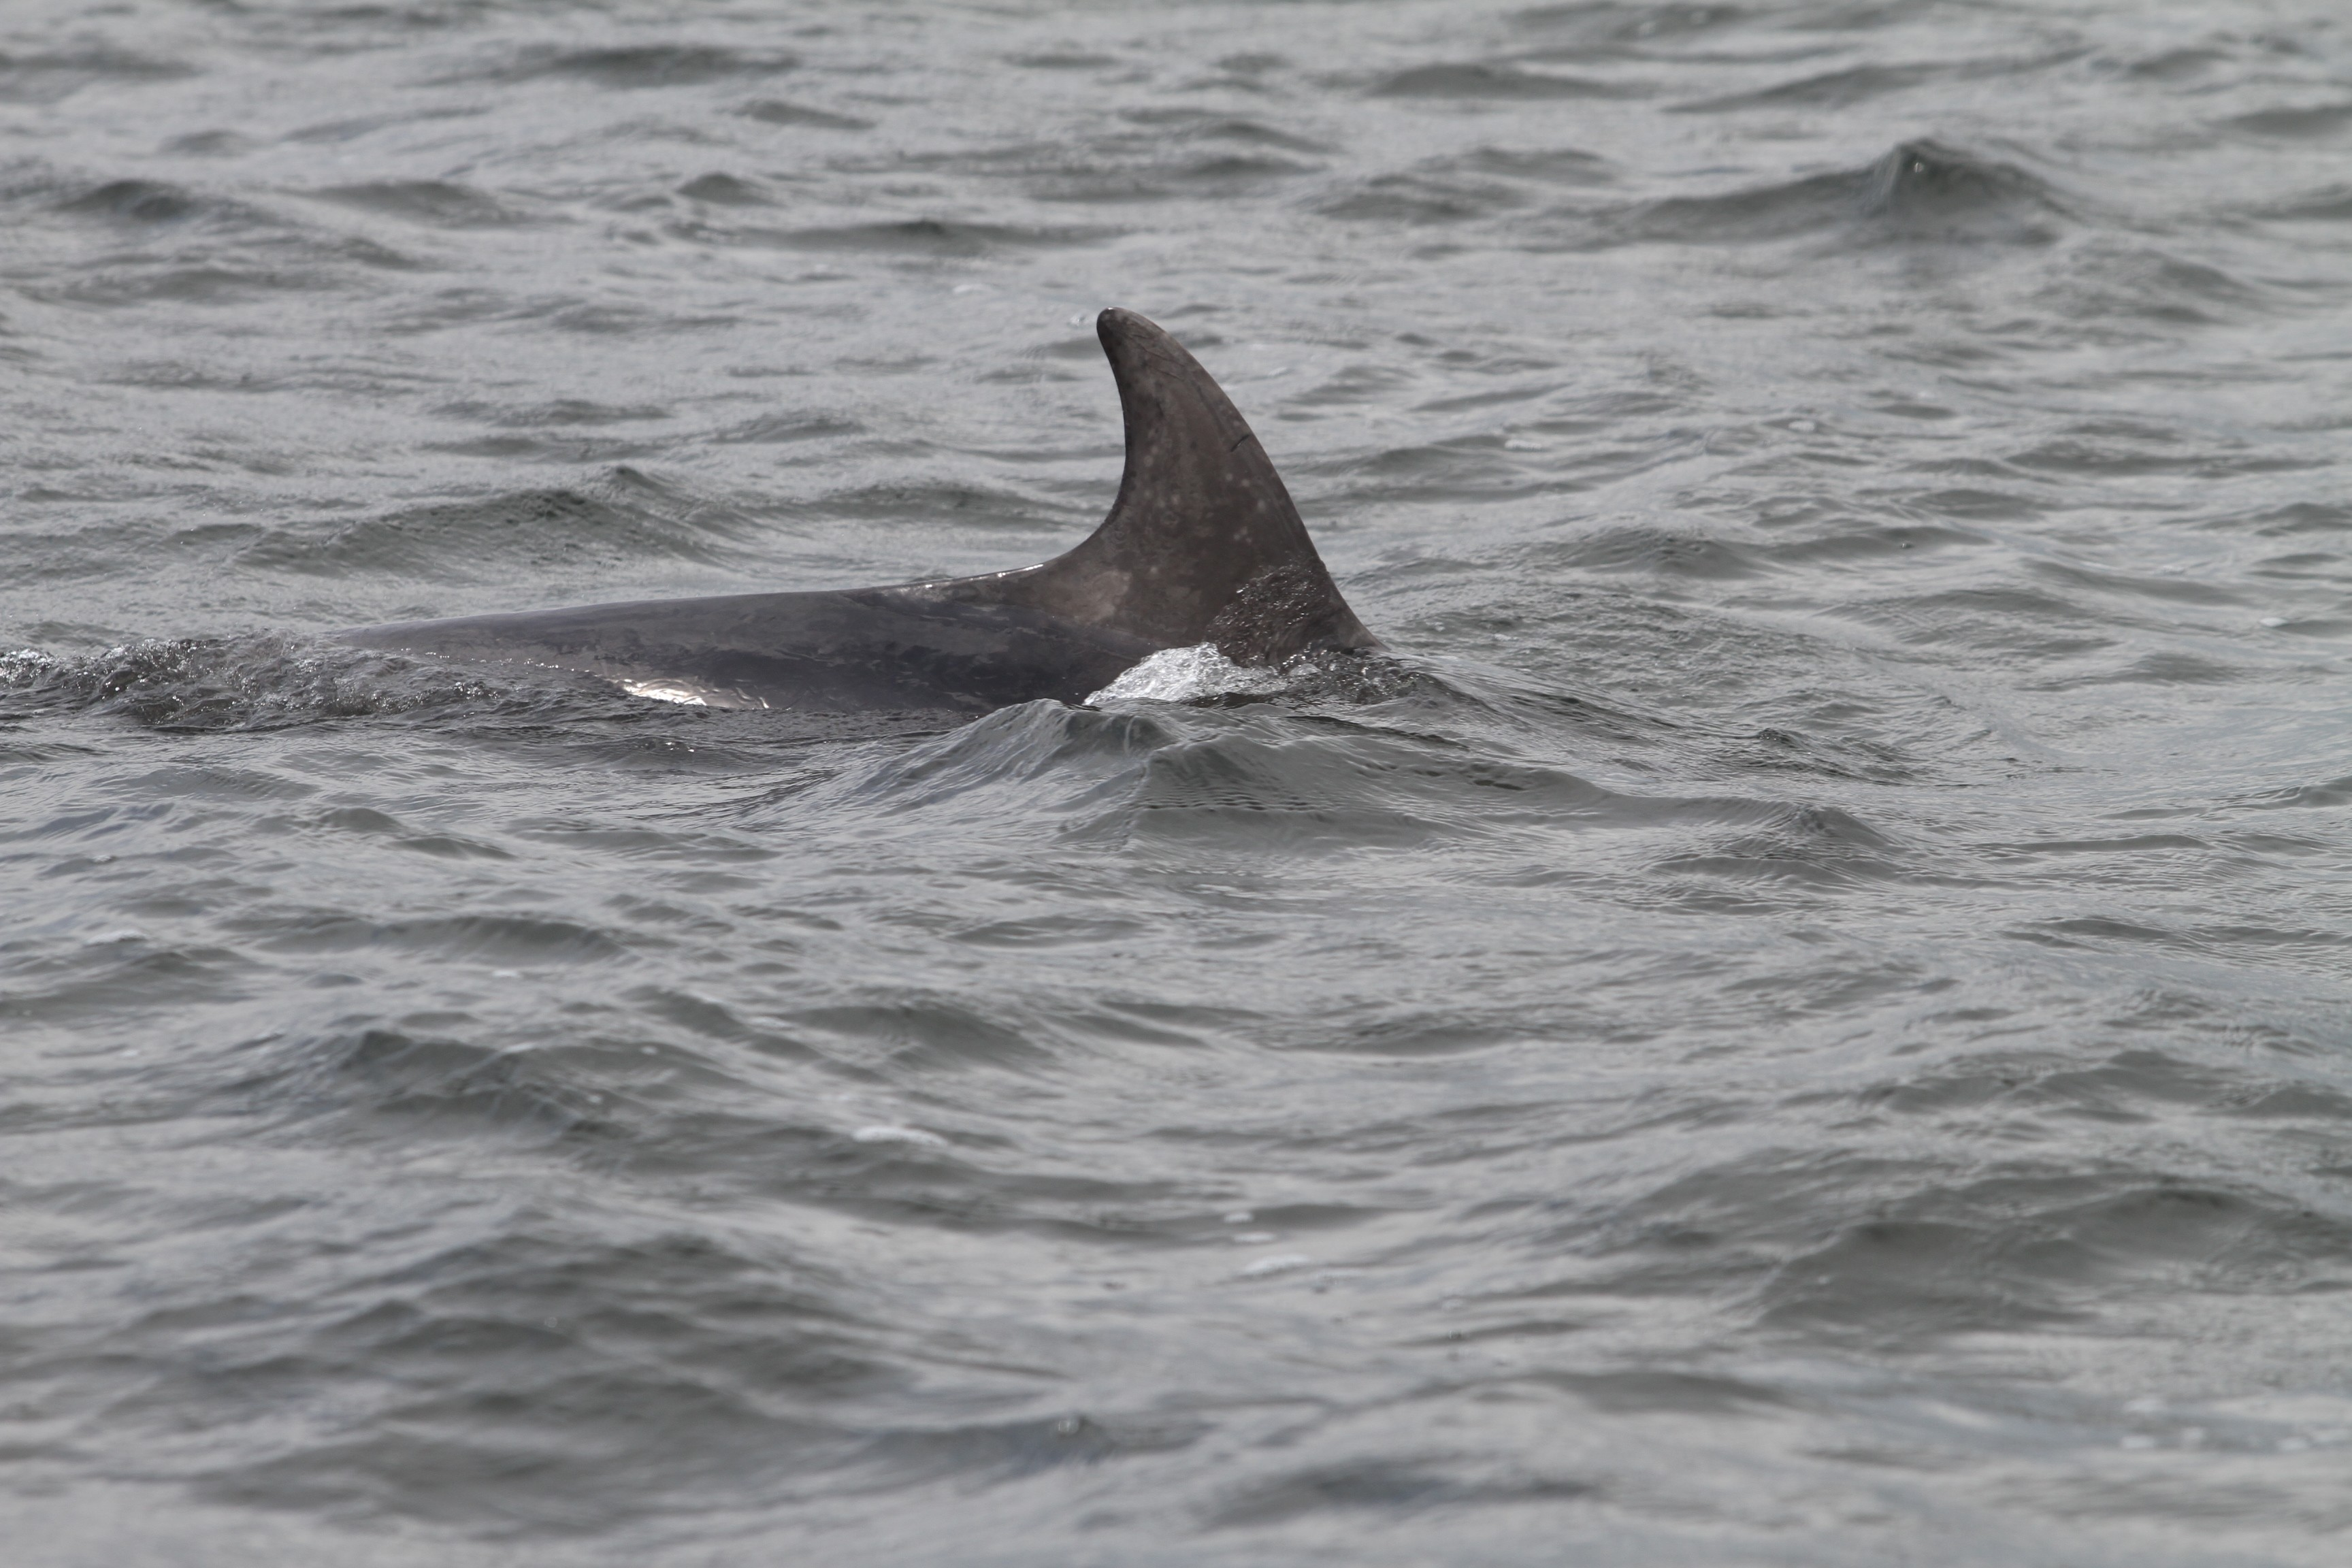
\includegraphics[width=0.8\textwidth]{example_train.jpg}
    \caption{Example image of a bottlenose dolphin}
    \label{fig:example_train}
\end{figure}

\begin{figure}
    \centering
    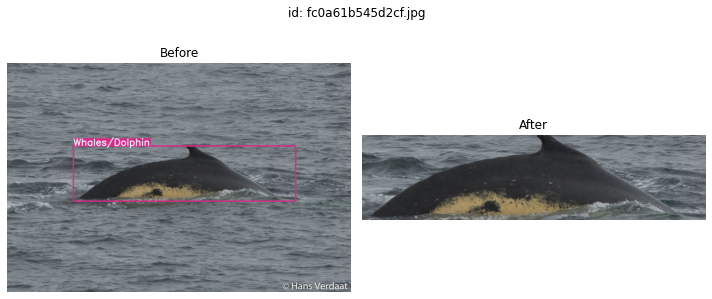
\includegraphics[width=0.8\textwidth]{image_cropping.png}
    \caption{Animal detection using YoloV5 model}
    \label{fig:image_cropping}
\end{figure}


The training images came in a variety of sizes. Figure \ref{fig:example_train} shows an example unprocessed image. Large amounts of each image are just of water which is irrelvant to the classification task. We are only interested in the parts of the 
images that contain the animals.

A solution to this issue was proposed within the discussions of the Kaggle competition \cite{cropped_dataset_kaggle}. YoloV5 was trained on a dataset of 1200 pictures of whale flukes and the corresponding location of points on the edge of the fluke for those pictures \cite{whale_fluke_dataset}. 
This was then assumed to generalise to finding the bounding box for any part of a whale or dolphin within the water. However, it is worth noting that finding the bounding box of any part of the animal is considered an Out of Distribution problem. From this technique a cropped dataset was created with all images having a dimension of 256 x 256. This is the dataset that was then used to train the whale 
and dolphin classifier.


\section {Image Transformation}

A custom PyTorch dataset class called \emph{WhaleDataset} was created for loading in the training images. One-hot encoding was used for the image lables, representing the individual ids provided.

The images were converted to RGB format as this was the compatible format for PyTorch. The images were then transformed using the TorchVision transforms package. The images were already all the same dimension from the preprocessing outlined in the previous section. 
The transformation involved convertsing the PIL image to a PyTorch tensor, scaling ther pixel values to the range [0,1] followed by normalizing the tensor by subtracting the mean and dividing by the standard deviation.

Scikit Learn's \emph{train\_test\_split} was used to split of 80/20 was used. A random state was specified for reproducability between training runs. Shuffling was enabled on the test set.

\section{Measuring Model Performance}

Performance of the model was measured via the Mean Average Precision @ 5 (MAP@5). Instead of using just accuracy as a measure, MAP@5 was used to account of the complexity of the
classification task. Accuracy only considers whether the top predicted class is correct or not. It does not take into account the ranking of predictions. 
MAP@5, on the other hand, considers the ranking of predictions within the top 5 predicted classes. It rewards models that rank the correct classes higher in the prediction list.

$$MAP@5 = \frac{1}{U} \sum_{u=1}^{U} \sum_{k=1}^{\min(n,5)} P(k) \times \text{rel}(k)$$

\begin{itemize}
    \item \verb|U| is the number of images 
    \item \verb|P(k)| is the precision at cutoff \verb|k|
    \item \verb|n| is an indicator function equaling 1 if the item at rank \verb|k| is the correct label, zero otherwise
\end{itemize}


\section{Network Architecture}

\begin{figure}
    \centering
    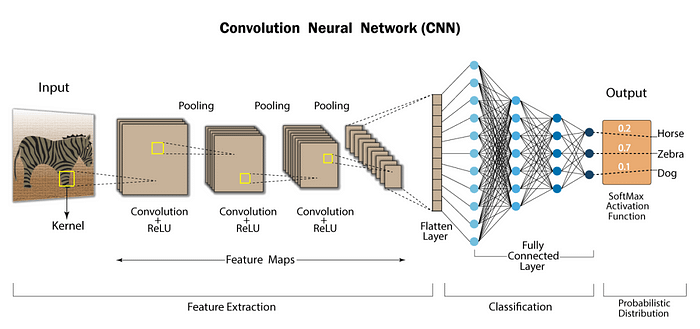
\includegraphics[width=0.8\textwidth]{cnn.png}
    \caption{Example of a CNN}
    \label{fig:network_architecture}
\end{figure}

A convolutional network architecture was selected for this problem. Three convolutional layers were selected for the network architecture so that increasingly more complex and 
abstract features could be extracted from the input image.

\begin{itemize}
    \item \verb|conv1|  takes the input image with 3 color channels (RGB) and applies 32 different 3x3 convolutional filters to extract low-level features like edges, corners, and simple patterns
    \item \verb|conv2| takes the output of the previous layer (32 feature maps) and applies 64 different 3x3 convolutional filters to detect slightly more complex patterns and features.
    \item \verb|conv3| takes the output of the previous layer (64 feature maps) and applies 128 different 3x3 convolutional filters to detect even more complex patterns and higher-level features that are useful for distinguishing between different classes.
\end{itemize}

After each convolutional layer, a ReLI activation function is applied to introduce non-linearity to the network


The first layer was a 2D Convultional layer. This layer takes the input image with 3 channels (RBG) and applies 32 different 3x3 convolutional filters to
extract low-level features like edges, corners and simple patterns. The stride of 1 ensures that the filters are applied to every pixel, and the 
padding of 1 preserves the spatial dimensionality. 

Next, a ReLU activation function was run to add non-linearity to the model followed by a pooling layer that downsamples the feature maps.

After the convolutional layers, there are two fully connected layers. The first fully connected layer takes the flattened output of the convolutional layers and applies a linear transformation, mapping to a fixed-sized vector of 512. his layer acts as a non-linear feature extractor, learning a higher-level representation of the convolutional features. A ReLU activation function is applied after this layer to introduce non-linearity.
The final fully connected layer applies a linear transformation, mapping the 512-dimensional vector to a vector of size equal to tthe number of unique individual\_ids in the training data.


\section{Model Training}

The Adam optimizer, a robust gradient-based optimization method. Adam allows for faster convergence, compared to stochastic gradient descent, by adapting the learing rate during training \cite{kingma2017adam}

Despite the massive reduction in file size that came from using the cropped dataset instead of the original dataset, training times on the local machine was still prohibitively long. Therefore, training was done using AWS Sagemaker using a ml.p3.8xlarge instance 


\section{Conclusions}

It has been shown that a 

\bibliographystyle{plain}
\bibliography{references}

\end{document}
